\section{Introduzione}

Il tool presentato in questo approccio affronta la necessità degli esperti di sicurezza di classificare le app come originali o offuscate. Per raggiungere questo obiettivo, il tool analizza il rapporto del numero degli stati dei metodi originali e il numero degli stati dei metodi in cui le azioni vengono sostituite con \textit{tau} (più dettagli in seguito), e inoltre analizza il rapporto tra i metodi validi e totali, e prova ad utilizzare queste informazioni per classificare le app come originali od offuscate. Il nostro lavoro ci ha permesso di giungere alla conclusione che il primo parametro non può essere utilizzato per fare questa classificazione, mentre il secondo può esserlo, consentendo di stabilire una soglia che discrimina le app originali da quelle offuscate.

\section{Tool}

Il nostro tool può essere eseguito sia su Windows 32 bit che su Linux 32/64 bit.

Lo pseudocodice del metodo principale del tool è il seguente:

\begin{myalgorithm}[caption={Pseudocodice metodo run()}, label={cod:pseudocodice-metodo-run}]
run() {
  if (!filesAlreadyProcessed()) {
    removeNonCcsFiles();

    distributeFilesToDirectories();

    fileNamesList = getFileNamesList();

    processFiles(fileNamesList);

    outputResults();
  }
}
\end{myalgorithm}

Le operazioni compiute da tali metodi sono:

\begin{itemize}
\item
\verb|if (!filesAlreadyProcessed())|: controlla che i file presenti nella cartella di analisi non siano stati già processati in una precedente esecuzione del tool;
\item
\verb|removeNonCcsFiles()|: rimuove i file diversi dal formato \verb|.ccs|, i quali non devono essere analizzati dal tool;
\item
\verb|distributeFilesToDirectories()|: distribuisce i file originali copiandoli in due directory, una per i file originali e una per i file modificati (quelli nei quali le azioni saranno sostituite con \textit{tau});
\item
\verb|fileNamesList = getFileNamesList()|: prende la lista dei file \verb|.ccs| e li memorizza in una lista di stringhe;
\item
\verb|processFiles(fileNamesList)|: processa i file, facendo la sostituzione con \textit{tau};
\item
\verb|outputResults()|: stampa in output i risultati dell'elaborazione.
\end{itemize}

Il metodo \verb|processFile()| elabora il singolo file \textit{.ccs} dato in input, calcolando le size del \textit{proc ALL} originale e del \textit{proc ALL} dei file modificati con la sostituzione di \textit{tau}:

\begin{myalgorithm}[caption={Pseudocodice metodo processFile()}, label={cod:pseudocodice-metodo-processfile}]
processFile(fileName) {
  filePath = getOriginalFilePathFromName(fileName);

  methodsList = getMethodsListInProcAll(filePath);

  for (method : methodsList) {
    processMethod(fileName, method);
  }

  // Compute 'sizeAll'
  originalFilePath = getOriginalFilePathFromName(fileName);
  int sizeAll = computeSizeAll(originalFilePath);

  // Compute 'sizeAllMin'
  modifiedFilePath = getModifiedFilePathFromName(fileName);
  int sizeAllMin = computeSizeAllMin(modifiedFilePath);

  // Add 'sizeAll' and 'sizeAllMin' to sum
  sumSizeAll += sizeAll;
  sumSizeAllMin += sizeAllMin;
}
\end{myalgorithm}

Nel metodo \verb|isMethodCallSequenceValid()| riportato di seguito analizziamo se un certo metodo presente nel \textit{proc ALL} presenta una sequenza di chiamate lineare. Con ``sequenza di chiamate lineare'' intendiamo dire una sequenza di chiamate di questo tipo:

\begin{myalgorithm}[caption={Modello di sequenza di chiamate lineari}, label={cod:modello-sequenza-di-chiamate-lineari}]
proc ALL = method1+[...]

proc method1 = action1.method2

proc method2 = action2.method3

...

proc methodN = actionN.nil
\end{myalgorithm}

Se la sequenza di chiamate è lineare, è possibile che il metodo sia offuscato (perché ha una struttura semplice). Il tool ci dà la possibilità di fissare una soglia massima di numero di stati del metodo, in modo da poter scegliere solo i metodi piccoli, o eventualmente di scegliere se prendere tutti i metodi (specificando una soglia altissima). Se la sequenza di chiamate è lineare ed è al di sotto della soglia, sostituiamo gli \verb|action1|, \verb|action2|, \dots, \verb|actionN| con \verb|t| (\textit{tau}).

Il metodo in questione è il seguente:

\begin{myalgorithm}[caption={Pseudocodice metodo isMethodCallSequenceValid()}, label={cod:pseudocodice-metodo-isMethodCallSequenceValid}]
isMethodCallSequenceValid(filePath, method) {
  // If the call has the form "return.nil" or "allreturn.nil"
  if (isMethodPassedAsArgumentEqualToNil(filePath, method)) {
    return true;
  }
  // If the instruction is 'invokeinit'
  else if (isInstructionEqualsToInvokeinit(filePath, method)) {
    return false;
  }
  // If the method call is linear
  else if (isMethodCallLinear(filePath, method)) {
    // Recursively call the method
    return isMethodCallSequenceValid(filePath, getMethodPassedAsArgument(filePath, method));
  }
  // Otherwise, if the method call is not linear
  else {
    return false;
  }
}
\end{myalgorithm}

In questo metodo controlliamo se la chiamata termina con \verb|.nil|: in tal caso sappiamo che siamo arrivati all'ultimo step della sequenza delle chiamate, e che anche questo step è lineare, quindi restituiamo \verb|true|. Invece, se l'azione è \verb|invokeinit|, dobbiamo escludere il metodo, perché si tratta di un metodo costruttore. Invece, se la chiamata in esame è lineare, chiamo ricorsivamente il metodo sullo step successivo della sequenza di chiamate (ossia, se la chiamata è del tipo \verb|proc method2 = action2.method3|, passo dall'analizzare \verb|method2| all'analizzare \verb|method3|). Infine, se la chiamata non ricade in nessuno dei casi precedenti, significa che la chiamata non è lineare, quindi restituisco \verb|false|.

\section{Metodologia}

Il nostro tool analizza il numero di stati del \textit{proc ALL} originale, ossia calcola la somma delle size dei singoli metodi del \textit{proc ALL} che hanno superato il test di linearità e che hanno la size inferiore o uguale alla soglia. Inoltre si effettua la minimizzazione del \textit{proc ALL} dei file nei quali è stata effettuata la sostituzione con \textit{tau}, tramite il comando \verb|min -S obseq ALL all_min|, e si calcola la size di \verb|all_min|. A questo punto si calcola la percentuale di riduzione tra i due valori, ossia, se con \verb|sizeAll| indichiamo la size del metodo \verb|ALL| originale e con \verb|sizeAllMin| indichiamo la size del metodo \verb|ALL| dei file modificati, la percentuale di riduzione è pari al valore:

\[ \text{percentualeRiduzione}\ = \frac{\text{sizeAll} - \text{sizeAllMin}}{\text{sizeAll}} \]

Ad esempio se il \textit{proc ALL} originale ha dimensione 100 e il \textit{proc ALL} modificato ha dimensione 80, la percentuale di riduzione sarà del:

\[ \text{percentualeRiduzione}\ = \frac{\text{100} - \text{80}}{\text{100}} = 20\% \]

La logica che ci ha portato a studiare questo parametro è l'ipotesi che, con l'introduzione di metodi offuscati, si vengono a creare tanti metodi ``vuoti'', che non fanno operazioni rilevanti, i quali vengono messi a \textit{tau} nella sostituzione. Quindi ci aspettiamo una percentuale di riduzione più elevata nell'app offuscata rispetto alla percentuale di riduzione nell'app originale.

Inoltre, il nostro tool valuta la percentuale dei metodi validi (ossia i metodi lineari che non contengono un \verb|invokeinit|)  rispetto ai metodi totali. Anche qui ci aspettiamo che questa percentuale sia maggiore per l'app offuscata, perché l'offuscamento introduce molti metodi che non fanno operazioni rilevanti e che hanno una forma lineare, il che porta ad un aumento del numero dei metodi validi.

\section{Risultati}

I risultati dell'analisi della percentuale di riduzione degli stati sono i seguenti:

\begin{figure}[H]
\centering
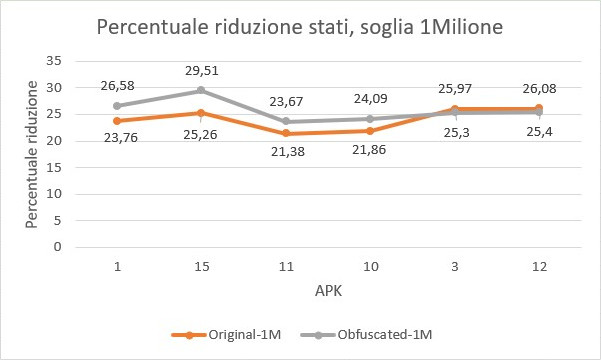
\includegraphics[width=0.88\textwidth]{img/risultati/stati_1M.jpg}
\caption{Percentuale di riduzione numero stati, soglia 1 milione.}
\label{fig:percentuale_riduzione_stati}
\end{figure}

Notiamo che non è possibile stabilire una soglia che discrimini le app originali dalle offuscate, perché, ad esempio, se prendiamo una soglia del 26,1\%, tutte le app originali sono al di sotto di questa soglia, però vi sono 4 app su 6 la cui versione offuscata è al di sotto di questa soglia, mentre dovrebbe essere al di sopra.

D'altra parte, analizzando il parametro della percentuale dei metodi validi rispetto ai metodi totali:

\begin{figure}[H]
\centering
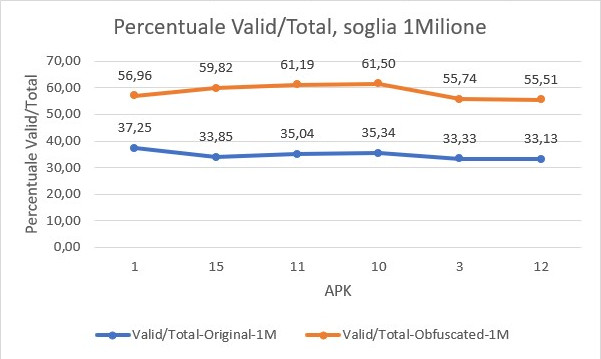
\includegraphics[width=0.88\textwidth]{img/risultati/metodi_1M.jpg}
\caption{Percentuale dei metodi validi rispetto ai metodi totali, soglia 1 milione.}
\label{fig:percentuale_metodi_validi}
\end{figure}

\noindent Notiamo che è possibile stabilire una soglia, pari al 46,38\%, che ci permette di discriminare le app originali dalle offuscate.

In conclusione, notiamo che il parametro della percentuale di riduzione del numero degli stati non può essere utilizzato per stabilire una soglia che discrimini le app originali dalle offuscate, mentre il parametro della percentuale dei metodi validi si presta allo scopo, sebbene esso non preveda l'utilizzo della riduzione in CWB-NC.